\section{System Evaluation}

\subsection{Evaluation Criteria}

In this section, the results of the simulation are presented. The randomised parallel algorithm proposed in \cite{yves2009optimal} is tested with three synchronization techniques using the simulator described previously. The theoretical bound for this algorithm is known to be $O(\log N)$. The synchronizers time and message complexity were discussed in section \ref{chap:3}. 

HERE INSERT DEFINITION OF TIME AND MESSAGES COMPLEXITY. CHECK IF THERE IS ALREADY IN THE INTRODUCTION.

 The aim of the simulation is to evaluate the time and message complexity of the algorithm. Additionally, show how the synchronization techniques generate overhead over the synchronous algorithm and present a discussion about the trade off between the techniques based on experimental results.


\subsection{Network Models}
\label{sec:topology}


The network topologies need to be generated before testing the \textit{MIS} algorithm. Topologies represent the distributed system in which the algorithm is going to be tested. Processors are mapped to vertices and the communication channels to edges.  The random graph model used to generate the networks topologies is the Stochastic Block Model (SBM), proposed in \cite{holland1983stochastic}.

Before entering in details on the SBM, a brief explanation about the Erd\~os--R\'enyi model is presented. This model is used to generate random graphs and it was first proposed in \cite{erdds1959random}. There are two variants of the model, in the $G(n, p)$ model a graph is constructed by connecting $n$ vertices randomly. An edge is included in the graph between two vertices $i,j$ with independent probability $p$. On \cite{erdos1960evolution} Erd\~os and R\'enyi presented some important properties about random graph. These properties about connectivity are used to generate the topologies for the simulations of this project and are cited below.


\begin{enumerate}
\item If $p<{\tfrac {(1-\epsilon )\ln n}{n}}$, then a graph $G(n, p)$ it is very likely to be disconnected.
\item If $p>{\tfrac {(1+\epsilon )\ln n}{n}}$ , then a graph $G(n, p)$ it is very likely to be connected.
\end{enumerate}

The most important point for this project is that ${\tfrac {\ln n}{n}}$ is a threshold of $p$ for generate graphs $G(n, p)$ that will almost surely be connected. 

In the SBM, the networks are characterised by blocks structures. Blocks define partitions of the networks, this means that vertices are associated in different subgroups and the distribution of the edges between vertices depend on the block in which a vertex is member. Assigning different probabilities to blocks, it is possible to obtain graphs that are denser in some regions. The probability for each group is defined in a probability matrix. In the next section, a formal definition of the \textit{SBM} is given with some examples of graphs generated by this model.

\subsection{Stochastic Block Model}

The SBM can be considered a probabilistic or generative model in which a probability is assigned to each pair of vertices $i,j$ in the network. This model define a probability distribution over networks $Pr(G | \theta)$, where $\theta$ are the parameters for the edges probabilities. For a given $\theta$, it is possible to generate a network instance G from the distribution by flipping a coin between every possible pair of vertices of the $G$. 

The Stochastic Block Model is defined by: 
\begin{enumerate}

    \item $k$: a scalar representing the number of blocks groups, clusters or modules in the network.
    \item $\overrightarrow{z}$: a vector of n element where $z(l)$ gives the block index of the vertex $l$.
    \item $M$ is a $k * k$ stochastic block matrix, where $M_{ij}$ gives the probability that a vertex of block type $i$ is connected to a vertex of block type $j$.
\end{enumerate}


The edges generated by flipping the coin between each pair of vertices are independent but not identically distributed. The large number of parameters allows the SBM  to produce very different structures. If $M_{ij} = p$ for each pair of blocks, then the SBM is reduced to the Erd\~os--R\'enyi model of random graph $G(n,p)$. The figure \ref{fig:erdos} show an example of stochastic block matrix in which every probability is the same for $k = 3$ blocks. Note that this is a square matrix and $k$ should be defined before $z$ and $M$. It can be seen that the probability distribution is the same for each block, as a consequence, the graph looks like one component even if the vertex belongs to different blocks types.

 In the figure \ref{fig:sbm}, another example of random graph is shown, however, in this example the probability distribution differ between blocks and it is more easy to visualize the different groups in the picture. The entrance $M_{i,j}$ where $i = j$ represent the probability of one edge between two vertices in the same group and the entrance $M_{i,j}$ where $i \neq j$ represent the probability of one edge between two vertices in the different groups. 

When $M_{i,i}$ is greater than $M_{i,j}$ for $i \neq j$ the vertices tend to connect other vertices that are in the same group. For this configuration the values of the diagonal are larger than values off it, in this case, it is the communities are assortative and the edges are more common within the blocks. On the contrary, on disassortative communities, edges between vertex of different communities are more common $M_{ii} <  M_{ij}$ for $i \neq j$.


Many other grouping criteria and variation of \textit{SBM} exist \cite{carrington2005models,holland1983stochastic,airoldi2008mixed}. Particularly, for this project, the assortative grouping is used for generating topologies from $N = 2^{6}$ to $2^{15}$ with power increments of 2 in the size of the network. The ${\tfrac {\ln n}{n}}$ threshold is used to set the probability of the diagonal in the matrix of probabilities. The values used in the parameters are similar to the used in \cite{kothapalli2013analysis}. 




\begin{figure}[ht]
\centering
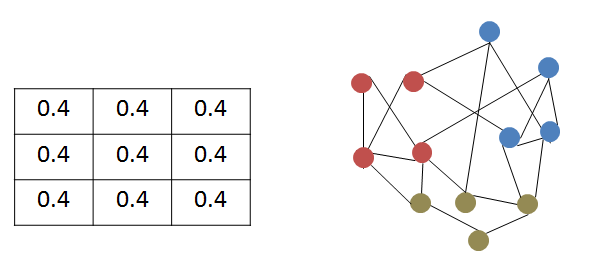
\includegraphics[width=1 \linewidth, height=5cm]{Erdos-Renyi.PNG} 
\caption{Example of SBM with equal probabilities}
\label{fig:erdos}
\end{figure}

\begin{figure}[ht]
\centering
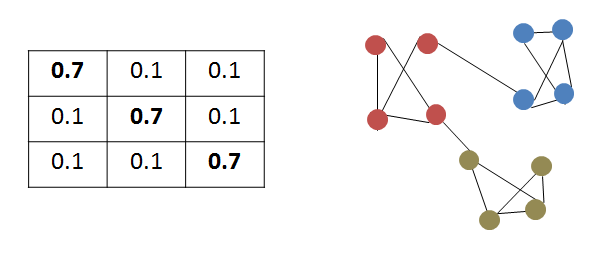
\includegraphics[width=1 \linewidth, height=5cm]{sbm.PNG} 
\caption{Example of SBM with assortative communities}
\label{fig:sbm}
\end{figure}

\subsection{Description of Experiments}

As mention in section \ref{chap:4}, the simulator was implemented in Elixir 1.6. The topology generator used to create network topology is an open source software written in Python under MIT license. Some modifications were done to the generator like generate the edges only for the triangular upper matrix, modified the number of clusters, customised the file format for topologies and some other minors modifications. The original code can be found here \url{https://github.com/tcoyze/stochastic-blockmodel} and the generator with the modification is inside the project repository.


The tests were run in a computer with processor Intel(R) Core(TM) i5--4210U of 1.7 and 2.4 GHz and RAM memory of 8 GB with additional 8 GB of SWAP. The operating system was a Linux 64 bit Debian base.

Regarding with network topologies, ten different topologies were generated with the Stochastic Block Model $G = (n,p)$ starting with $n=64,256,512,...,32768$. The number of blocks $k$ is set to $\log n$. The value used for the probability $p$ on the diagonal of the block matrix was $7{\tfrac {\ln n}{n}}$  and for values out of the diagonal $p\prime = {\tfrac {10}{n}}$. The value for $p$ was chosen to make sure that the generated graph is connected. Note that the algorithm for \textit{MIS} does not require this condition because it still reaches the solution even if the graph is disconnected. However, the Beta Synchronizer construct a rooted spanning tree over the topology in order to send \textbf{safe} and \textbf{go} messages to the root and from it. Because of this, if the topology is not connected the rooted spanning tree can not be constructed.


For each topology, the results presented are the average 10 executions of the simulation. For the \textit{MIS } algorithm it is desirable to measure the average because the randomised nature of the algorithm and the unpredictable behaviour of the asynchronous message passing at the bottom. In consequence, for a given topology it is possible to obtain different results. The results observed in the simulation show that the number of rounds is similar in different execution however in can be some important differences in the number of messages. These results are presented in the next section.

The steps to perform the experiments are enumerate below:

\begin{enumerate}
\item Implementation of the synchronizers Alpha and Beta.
\item Implementation of the Maximal Independent Set algorithm using the simulation developed in step 1.
\item Implementation of the Maximal Independent Set Algorithm using a global synchronization technique.
\item Create the topology with the Stochastic Block Model according to the description in the section \ref{sec:topology}.
\item Run N times the synchronous algorithm for the \textit{MIS} and saves the results for each synchronizer technique (Alpha, Beta and Global).
\item Compute the average and present the results.
\end{enumerate}




